\documentclass[11pt]{article}
\usepackage[margin=2.5cm]{geometry}
\usepackage{booktabs}
\usepackage{pgfplots}
\pgfplotsset{compat=1.17}
\usepackage{caption}

\title{Rare-number crowding across pretraining checkpoints}
\author{}
\date{}

\begin{document}
\maketitle

\noindent For each training checkpoint we take the rarest and the most frequent tenth of four-digit numbers
(200 numbers each, matched for magnitude and digit form), compute their persistence barcode at $\sim$84\% depth,
and report the mean H0 death (mean gap between neighbouring numbers). The ratio rare/frequent removes the overall
change in scale during training: $1$ means no difference, values below $1$ mean rare numbers are more crowded.

\begin{table}[ht]
\centering
\small
\begin{tabular}{rrrr}
\toprule
Step & Rare & Frequent & Rare / Freq. \\
\midrule
0 & 4.98 & 4.99 & 0.998 \\
64 & 4.51 & 4.53 & 0.997 \\
256 & 4.78 & 4.84 & 0.988 \\
512 & 6.06 & 6.36 & 0.953 \\
1{,}000 & 19.03 & 18.63 & 1.021 \\
2{,}000 & 25.32 & 26.00 & 0.974 \\
4{,}000 & 39.41 & 40.33 & 0.977 \\
8{,}000 & 65.02 & 67.03 & 0.970 \\
13{,}000 & 79.25 & 82.31 & 0.963 \\
23{,}000 & 94.20 & 98.15 & 0.960 \\
33{,}000 & 94.58 & 97.20 & 0.973 \\
53{,}000 & 89.19 & 90.84 & 0.982 \\
73{,}000 & 83.66 & 85.09 & 0.983 \\
103{,}000 & 64.84 & 65.49 & 0.990 \\
123{,}000 & 60.06 & 60.77 & 0.988 \\
143{,}000 & 55.10 & 56.05 & 0.983 \\
\bottomrule
\end{tabular}
\caption{Pythia-1.4B: mean H0 death of the rarest and the most frequent tenth of four-digit numbers
(matched for magnitude and digits) at $\sim$84\% depth, across training. Ratio $<1$: rare numbers are more crowded.}
\label{tab:ckpt_pythia}
\end{table}

\begin{table}[ht]
\centering
\small
\begin{tabular}{rrrr}
\toprule
Step & Rare & Frequent & Rare / Freq. \\
\midrule
0 & 207.82 & 209.51 & 0.992 \\
300 & 138.16 & 137.69 & 1.003 \\
10{,}000 & 82.59 & 85.13 & 0.970 \\
20{,}000 & 57.35 & 59.33 & 0.967 \\
40{,}000 & 32.36 & 33.95 & 0.953 \\
70{,}000 & 18.35 & 19.03 & 0.964 \\
140{,}000 & 15.28 & 15.75 & 0.970 \\
250{,}000 & 13.95 & 14.29 & 0.976 \\
420{,}000 & 13.29 & 13.74 & 0.967 \\
710{,}000 & 12.16 & 12.45 & 0.976 \\
1{,}170{,}000 & 12.58 & 12.83 & 0.981 \\
1{,}907{,}359 & 13.57 & 13.82 & 0.982 \\
\bottomrule
\end{tabular}
\caption{OLMo-2-1B: as Table~\ref{tab:ckpt_pythia}.}
\label{tab:ckpt_olmo}
\end{table}

\begin{figure}[ht]
\centering
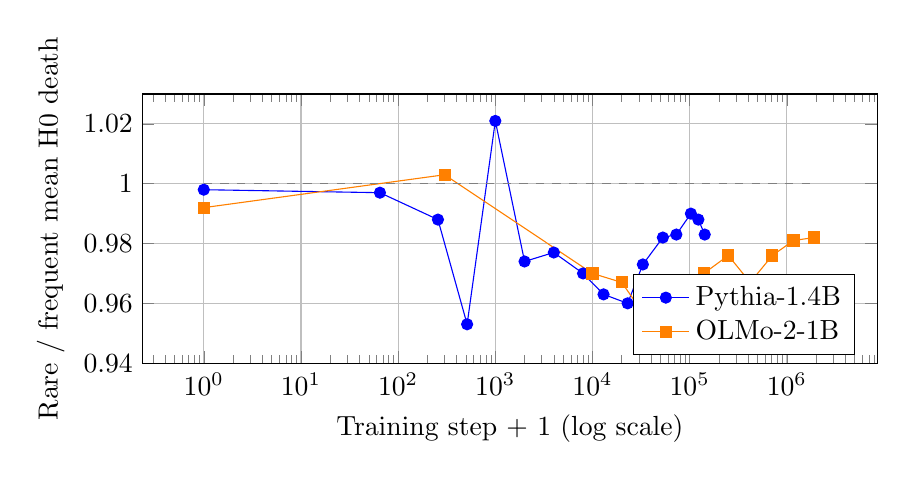
\begin{tikzpicture}
\begin{semilogxaxis}[
  width=0.9\linewidth, height=5cm,
  xlabel={Training step + 1 (log scale)}, ylabel={Rare / frequent mean H0 death},
  ymin=0.94, ymax=1.03, grid=major, legend pos=south east, legend cell align=left]
\addplot[mark=*, blue] coordinates {
 (1,0.998) (65,0.997) (257,0.988) (513,0.953) (1001,1.021) (2001,0.974) (4001,0.977) (8001,0.970)
 (13001,0.963) (23001,0.960) (33001,0.973) (53001,0.982) (73001,0.983) (103001,0.990) (123001,0.988) (143001,0.983)};
\addlegendentry{Pythia-1.4B}
\addplot[mark=square*, orange] coordinates {
 (1,0.992) (301,1.003) (10001,0.970) (20001,0.967) (40001,0.953) (70001,0.964) (140001,0.970)
 (250001,0.976) (420001,0.967) (710001,0.976) (1170001,0.981) (1907360,0.982)};
\addlegendentry{OLMo-2-1B}
\addplot[dashed, gray, domain=1:2000000] {1};
\end{semilogxaxis}
\end{tikzpicture}
\caption{Rare-number crowding across training ($\sim$84\% depth): $1$ = no difference, $<1$ = rare numbers more crowded.}
\label{fig:ckpt_ratio}
\end{figure}

\end{document}
